\chapter{Methods}
\label{chp:methods}

\begin{center}
    \textit{This chapter outlines the development process, including the design and implementation of the application, tools and framework used, and testing strategies.}
\end{center}


\section{Machine Learning Models}
\label{sec:ml-models}

As mentioned in the theory chapter, ChessCam is an open-source tool for digitizing chess games using visual recognition. During the early development phase, this project was revisited in greater depth and ultimately chosen as the foundation for the machine learning component. It employs two \glspl{cnn}, one for detecting chess pieces and another for locating the squares of the chessboard \cite{github:chesscam}. While the documentation was limited, the core logic and structure of the models were accessible in the repository. For any unclear aspects, communication with the developers helped ensure a correct understanding of the models. \\

The ChessCam repository offered models in multiple formats, including PyTorch and \gls{onnx}. To integrate them into the project, it was first necessary to understand the expected inputs and outputs. Netron was used to inspect and understand the models.


\subsection{Piece Detection Model}
The piece detection model was responsible for identifying and classifying chess pieces on the board. It expected \textbf{input} in the format \textbf{[1, 3, 288, 480]}. \textbf{1} represented the batch size, i.e. the number of images processed at once. \textbf{3} corresponded to the number of color channels (RGB), indicating that the image had to be in color. \textbf{288} and \textbf{480} denoted the height and width of the image in pixels, respectively. \\

The piece model output data in the format \textbf{[1, 16, 2835]}. \textbf{1} represented the batch size. \textbf{2835} represented the number of anchor boxes used in the detection and \textbf{16} consisted of two parts: \\

The first 4 values were offset values that adjusted the position and size of each anchor box to better align with a detected piece. These offsets were relative to the predefined anchor boxes, as illustrated in Table \ref{tab:piece-offset-table}.

\begin{table}[h]
    \centering
    \caption[Offset values for anchor boxes (chess pieces)]{Example offset coordinates for each anchor box with regard to identifying chess pieces.}  % Caption moved to top
    \renewcommand{\arraystretch}{1.3} % Increase row height to allow text to be on top
    \begin{tabular}{lcccc}
        \toprule
        \textbf{Anchor box} & \textbf{xcenter} & \textbf{ycenter} & \textbf{width} & \textbf{height} \\
        \midrule
        Anchor box 1 & -3.23 & 0.57 & -0.12 & -0.34 \\
        Anchor box 2 & 0.51 & -0.63 & 4.15 & 1.27 \\
        Anchor box 3 & 7.71 & 0.29 & -0.11 & 2.45 \\
        ... & ... & ... & ... & ... \\
        Anchor box 2835 & -0.04 & 2.11 & 1.15 & 5.32 \\
        \bottomrule
    \end{tabular}
    \label{tab:piece-offset-table}
\end{table}


The remaining 12 values represented the probabilities for each possible piece type after the offset value had been applied. With 12 different piece types, the model output 12 probabilities for each anchor box. The classification labels are shown in Table \ref{tab:piece-label-table}. Table \ref{tab:piece-probability-table} presents the predicted probabilities for each label across all anchor boxes. \\

\vspace{2mm}

\begin{table}[ht]
\renewcommand{\arraystretch}{1.1}  % Increase row height slightly
\centering
\caption[Labels for chess piece types]{List of predefined class labels corresponding to the 12 chess piece types used for model classification.}
\begin{tabular}{|c|c|}
\hline
\multicolumn{2}{|c|}{\textbf{Model Labels}} \\  
\hline
\textbf{Black Pawn} & \textbf{White Pawn} \\
\textbf{Black Knight} & \textbf{White Knight} \\
\textbf{Black Bishop} & \textbf{White Bishop} \\
\textbf{Black Rook} & \textbf{White Rook} \\
\textbf{Black Queen} & \textbf{White Queen} \\
\textbf{Black King} & \textbf{White King} \\
\hline
\end{tabular}
\label{tab:piece-label-table}
\end{table}


\begin{table}[h]
    \centering
    \caption[Predicted chess piece after applying offset]{Predicted class probabilities for each anchor box after applying the offset.}  % Caption moved to top
    \renewcommand{\arraystretch}{1.3}
    \begin{tabular}{lcccc}
        \toprule
        \textbf{Anchor box} & \textbf{Black Pawn} & \textbf{White Pawn} & \textbf{Black Knight} & \textbf{...} \\
        \midrule
        Anchor box 1 & \raggedright 0.03 & \raggedright 0.71 & \raggedright 0.01 & ... \\
        Anchor box 2 & \raggedright 0.82 & \raggedright 0.02 & \raggedright 0.01 & ... \\
        Anchor box 3 & \raggedright 0.02 & \raggedright 0.01 & \raggedright 0.78 & ... \\
        ... & ... & ... & ... & ... \\
        Anchor box 2835 & \raggedright 0.01 & \raggedright 0.03 & \raggedright 0.05 & ... \\
        \bottomrule
    \end{tabular}
    \label{tab:piece-probability-table}
\end{table}

\newpage

There were 2835 predefined anchor boxes spread across the image, each serving as a candidate location for detecting a chess piece. During training, the model learned to adjust these anchor boxes to better match the actual pieces on the board. It achieved this by predicting 4 offset values that modified the location and size of each anchor box. At runtime, for each anchor box, the model used these learned offsets and output 12 class probabilities, indicating the likelihood of each chess piece type being present at that location.

\subsection{XCorners Detection Model}
The corner detection model identified the points where the edges of the inner squares on the chessboard met, referred to as \textit{intersection points} or \textit{xcorners}. Up to 49 intersection points could be detected in a single image. These points are illustrated in Figure \ref{fig:xcorners-chessboard}.

\begin{figure}[h!]
    \centering
    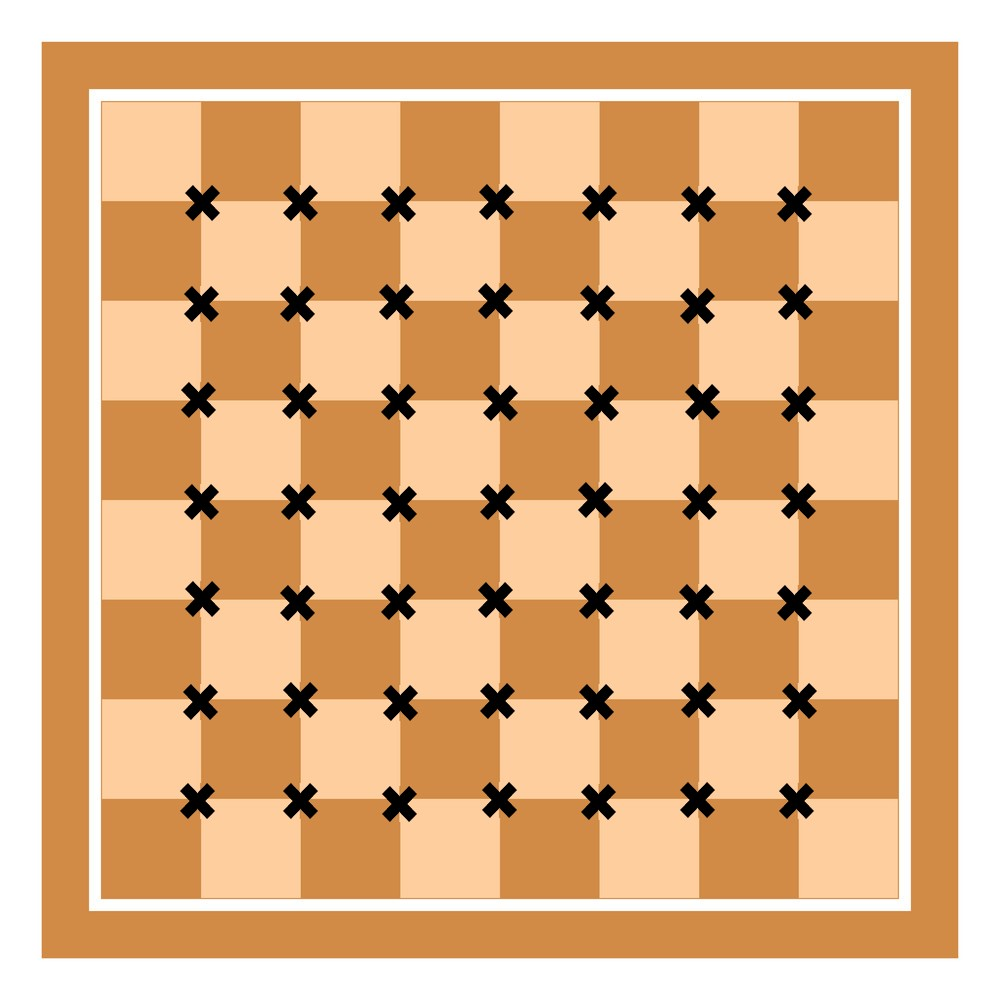
\includegraphics[width=0.75\linewidth]{figures/methods/ml-models/xcorners_chessboard.jpg}
    \caption[Detected intersection points on chessboard]{Visualization of intersection points where the edges of the inner squares on the chessboard meet. The model identified and predicted these points. Up to 49 intersection points could be detected in a single image \cite{vectorstock:chessboard-svg}.}
    \label{fig:xcorners-chessboard}
\end{figure}

The input for the corner model was the same as the piece model: \textbf{[1, 3, 288, 480]}. The corner model output predictions in the format \textbf{[1, 5, 2835]}. \textbf{1} represented the batch size. \textbf{2835} represented the number of anchor boxes used in the detection and \textbf{5} consisted of two parts: \\

\newpage

The first 4 values were offset values that adjusted the position and size of each anchor box, aligning it more accurately with a potential intersection point. These offsets were relative to the original anchor box coordinates, as shown in Table \ref{tab:corner-offset-table}.

% \newpage

\begin{table}[h]
    \centering
    \caption[Offset values for anchor box (intersection points)]{Example offset coordinates for each anchor box with regard to identifying intersection points.}  % Caption moved to top
    \renewcommand{\arraystretch}{1.3} % Increase row height to allow text to be on top
    \begin{tabular}{lcccc}
        \toprule
        \textbf{Anchor box} & \textbf{xcenter} & \textbf{ycenter} & \textbf{width} & \textbf{height} \\
        \midrule
        Anchor box 1 & -1.43 & 3.27 & -0.52 & -2.21 \\
        Anchor box 2 & 2.51 & -7.61 & 0.15 & 4.17 \\
        Anchor box 3 & -3.71 & 1.49 & -4.21 & 2.45 \\
        ... & ... & ... & ... & ... \\
        Anchor box 2835 & -2.04 & 3.29 & -0.35 & 1.24 \\
        \bottomrule
    \end{tabular}
    \label{tab:corner-offset-table}
\end{table}

The final value was the probability that the adjusted anchor box corresponded to an intersection point on the chessboard, as illustrated in Table~\ref{tab:corner-probability-table}. \\

\begin{table}[h]
    \centering
    \caption[Predicted intersection points after applying offset]{Predicted intersection probabilities for each anchor box after applying the offset.}
    \renewcommand{\arraystretch}{1.3}
    \begin{tabular}{lc}
        \toprule
        \textbf{Anchor Box} & \textbf{Intersection Probability} \\
        \midrule
        Anchor Box 1 & 0.06 \\
        Anchor Box 2 & 0.91 \\
        Anchor Box 3 & 0.03 \\
        ... & ... \\
        Anchor Box 2835 & 0.87 \\
        \bottomrule
    \end{tabular}
    \label{tab:corner-probability-table}
\end{table}


% \newpage


\subsection{Combining The Models}

To track chess piece movements, the process began with identifying the individual squares of the chessboard. Achieving this required first determining the outer corners of the board, which served as reference points for constructing the grid. Once the corners were located, the chessboard could be subdivided into an 8×8 grid of uniformly sized squares. Given the known distances between the corners and the regular structure of the board, the center point of each square could be accurately calculated. These center points were then used as the basis for mapping each detected piece to a specific square, as illustrated in Figure~\ref{fig:chessboard-centers}.

\newpage



\begin{figure}[h!]
    \centering
    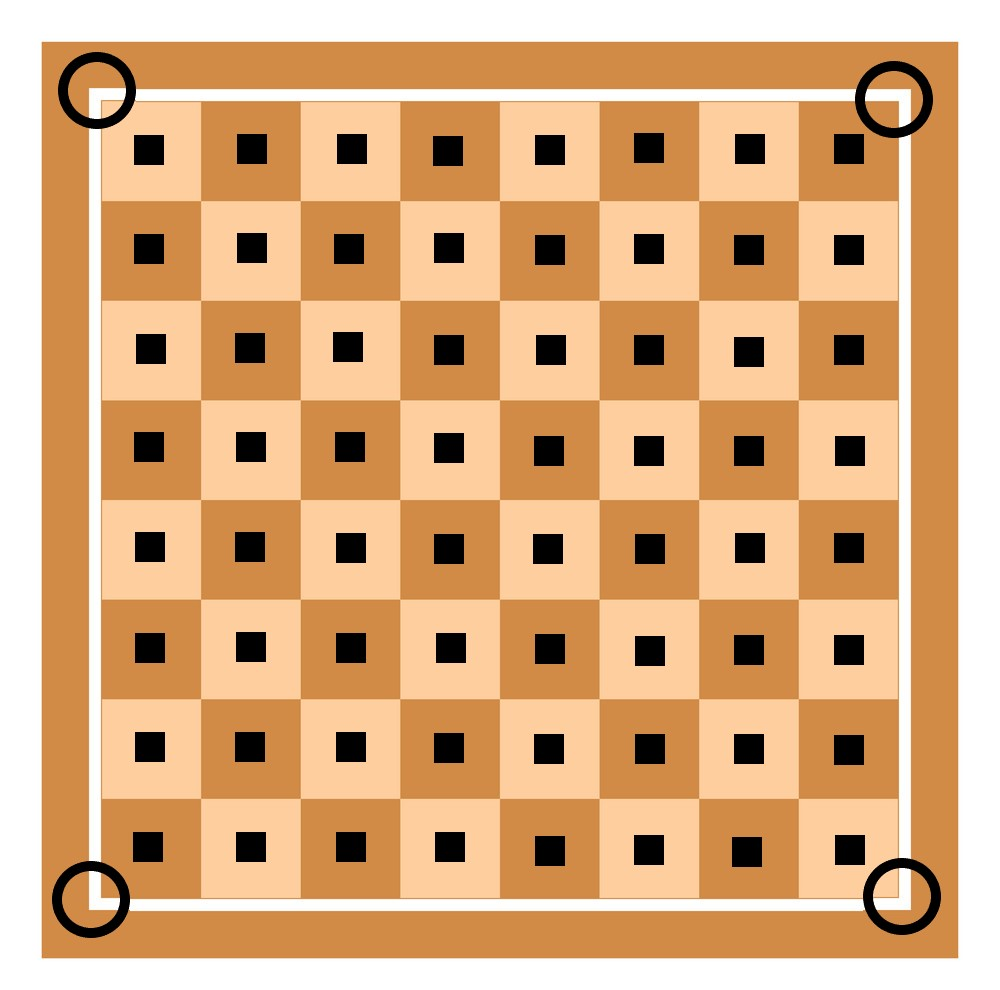
\includegraphics[width=0.75\linewidth]{figures/methods/ml-models/outer_corners_centers_chessboard.jpg}
    \caption[Chessboard corners and centers]{Visualization of the corners of the chessboard and the centers of each individual square \cite{vectorstock:chessboard-svg}.}
    \label{fig:chessboard-centers}
\end{figure}


The bottom center of each piece’s bounding box was selected as its representative location, as highlighted in Figure~\ref{fig:bbox-black-pawn}. Each detected piece was then mapped to the nearest square center based on the minimum Euclidean distance, as described in Section \ref{subsec:euclidean-distance}. This approach made it possible to accurately assign each piece to a specific square on the chessboard.


% \newpage


\begin{figure}[h!]
    \centering
    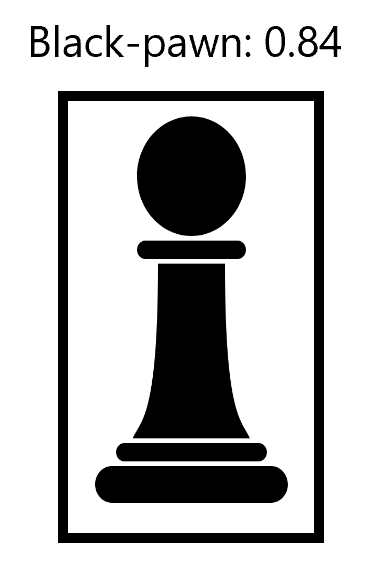
\includegraphics[width=0.25\linewidth]{figures/methods/ml-models/black-pawn.png}
    \caption[Detected chess piece and its bounding box]{Example of a detected chess piece with its classification confidence score. The bottom center of the bounding box was used as the reference point for mapping the piece to its corresponding square \cite{svgrepo:black-pawn-svg}.}
    \label{fig:bbox-black-pawn}
\end{figure}


\subsubsection*{Board Detection}

Each frame captured by the camera was processed by the two models. Before inference, the frame had to match the models’ expected input dimensions [1, 3, 288, 480]. This process included scaling the frame, normalizing the pixel values to fall within the range [0, 1], and converting the image to the appropriate data type. \\

After inference, the models produced the prediction outputs: [1, 16, 2835] for pieces and [1, 5, 2835] for intersection points. To identify the most reliable predictions, low-confidence entries were first filtered out. Furthermore, \gls{nms} was applied to further refine the results. This process ensured only the most accurate locations for the pieces and intersections were retained. \\

To identify the board corners of the chessboard, Delaunay triangulation was used, as described in Section \ref{subsec:delaunay-triangulation}. Delaunay triangulation was applied to the intersection points to generate a set of candidate triangles. By iterating over these triangles and examining their shared vertices, the algorithm identified potential quadrilaterals (four-sided shapes) that represented the four corners of the chessboard. Once a list of candidate quadrilaterals was generated, each was scored based on how well it fit the original intersection points. The quadrilateral with the highest score was then selected as the most likely representation of the board corners. \\

With the corners identified, the next step was to correct the distortion caused by the camera angle. When viewed at an angle, the board appeared skewed due to varying distances between the camera and different parts of the board. This distortion was corrected by using a perspective transformation. Specifically, the inverse of the transformation matrix responsible for the distortion was computed. By applying this inverse to the distorted image, the transformation that warped the image was reversed, effectively 'flattening' the distorted chessboard back to its ideal, top-down view. Once the inverse matrix was applied, the resulting coordinates provided the corrected positions of the corners in the distorted image. \\

With the distortion corrected, the board was treated as an 8×8 grid of uniformly sized squares, each occupying a unit-length cell. The center of each square lies midway between its edges, resulting in center coordinates that ranged from 0.5 to 7.5 in both the x and y axes. The center of the first square was at (0.5, 0.5), the second at (1.5, 0.5), and so on up to (7.5, 7.5). \\

To finalize the board orientation, the average center of all black and white pieces was computed. The board was then rotated in four 90-degree increments. For each rotation, the midpoints of the expected white and black sides were calculated as the average coordinates between pairs of corners. Specifically, the midpoint for the white side was calculated between ‘a1’ and ‘h1’, and for the black side between ‘a8’ and ‘h8’. The rotation that minimized the distance between piece centers and these midpoints was selected as the correct alignment. Based on this orientation, the labels ‘a1’, ‘h1’, ‘a8’, and ‘h8’ were assigned to the corners of the chessboard. A visualization of this process is shown in Figure \ref{fig:board_label_assignment}.

\begin{figure}[h!]
\centering
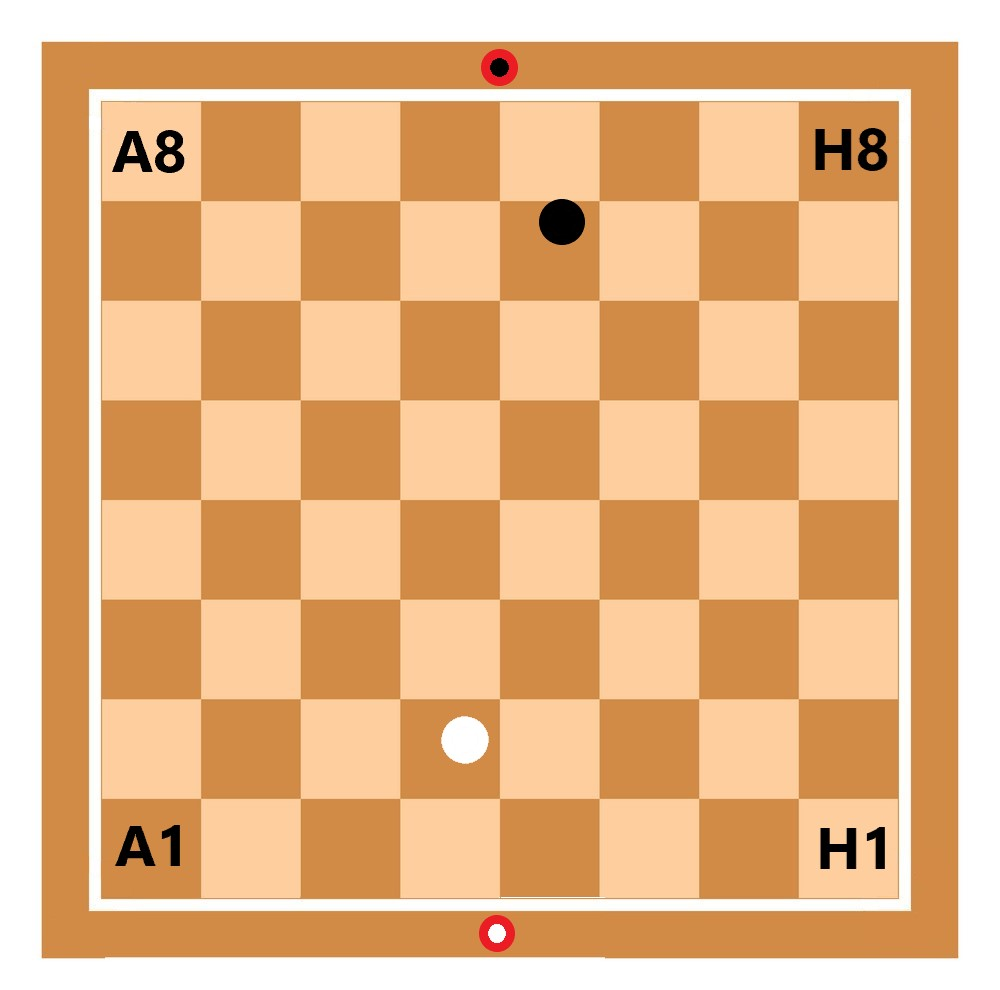
\includegraphics[width=0.70\linewidth]{figures/methods/ml-models/label_assignment_board.jpg}
\caption[Assigning labels to chessboard]{The white and black circles represent the average centers of the white and black pieces. The red circles indicate the midpoints between the corners on the white and black sides.  \cite{vectorstock:chessboard-svg}.}
\label{fig:board_label_assignment}
\end{figure}



\subsubsection*{Move detection}

After detecting the chessboard and pieces, the application continuously processed each incoming video frame to determine whether a move had occurred. For every frame, the internal board state was updated based on the observed positions of the chess pieces. \\

To ensure stability, the system used a decay-based mechanism that blended the current detections with the previous state. This approach helped smooth out transient errors caused by occlusions or momentary inconsistencies in the video feed. Additionally, updates were throttled to fixed intervals, reducing computational overhead and avoiding unnecessary changes due to minor fluctuations in detection. \\

Once the updated board configuration was determined, it was compared to the set of legal moves for the current state. If a high-confidence legal move was identified, it was registered and applied. The move was then committed to the internal board state and sent to the frontend via the WebSocket connection to support ongoing analysis and visualization.

\newpage

\subsubsection*{Pre-recorded video}

To streamline the development of the machine learning model, prerecorded video footage was used instead of a live camera feed. This approach provided a consistent and controlled environment where the model could be developed and refined by replaying the same chess game repeatedly. Using static video eliminated the need to physically set up the chessboard and camera for each iteration, significantly speeding up the development process. \\

\begin{figure}[h!]
    \centering
    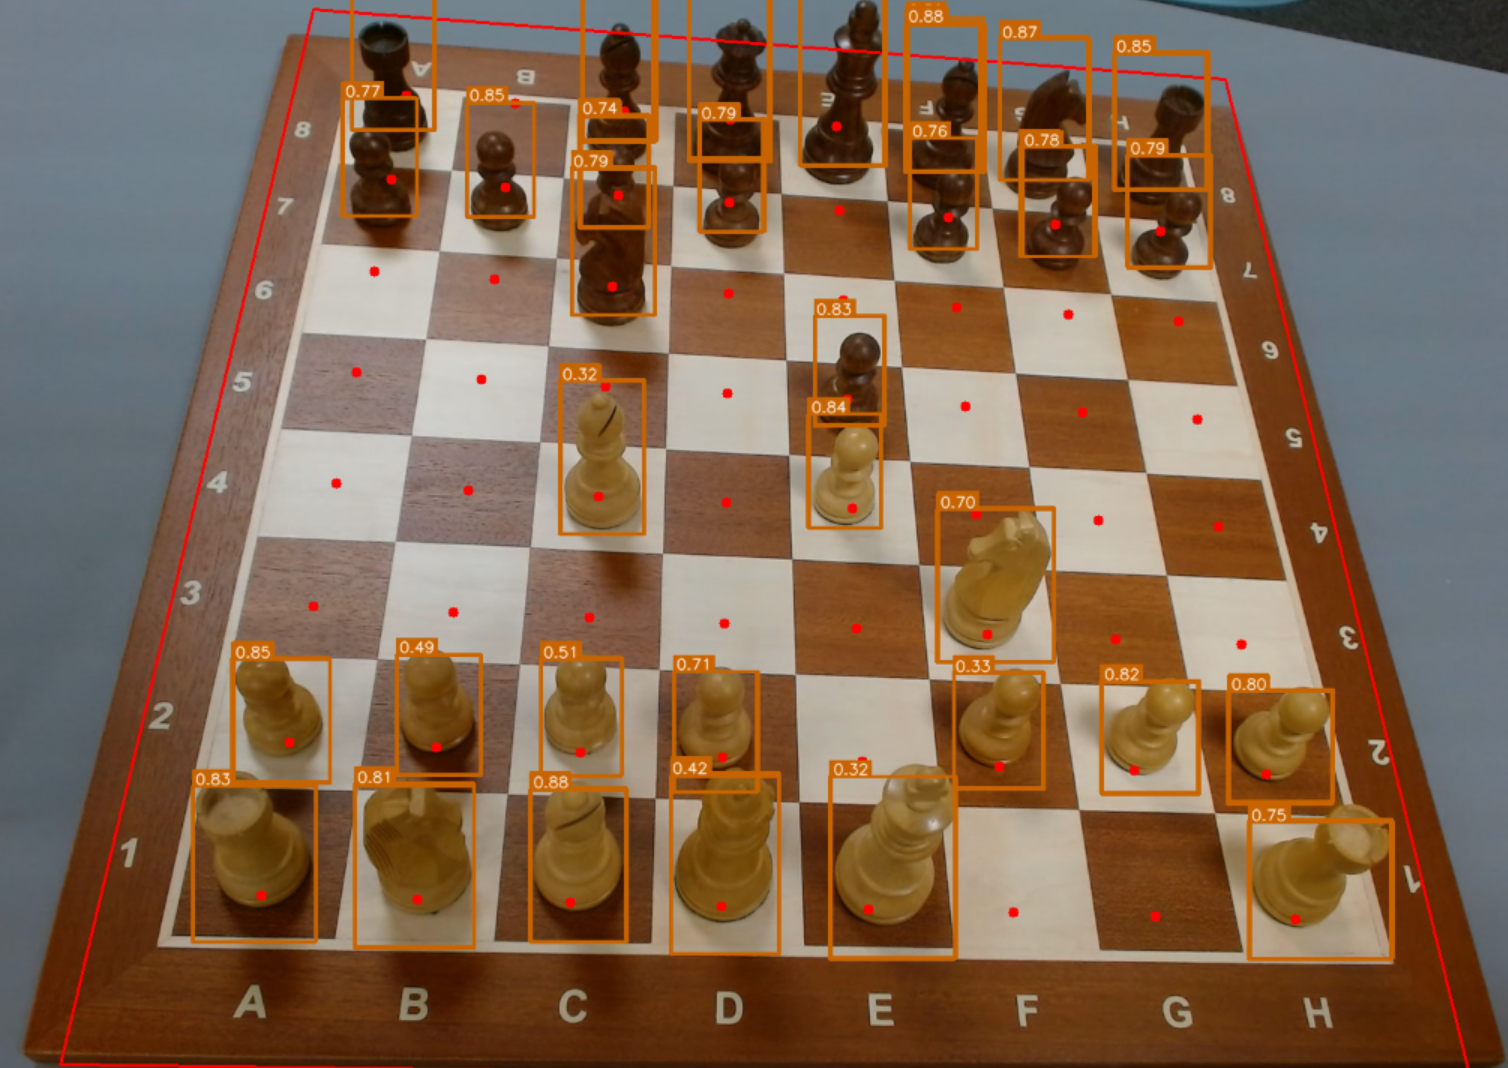
\includegraphics[width=0.75\linewidth]{figures/methods/ml-models/piece-model.png}
    \caption[Visualization of piece model and corner model]{Visualization of the detected pieces and centers of the squares.}
    \label{fig:websocket-vs-http}
\end{figure}

\section{Design}
\label{subsec:wireframe}

\subsubsection*{Control Panel}

The Control Panel is a desktop interface for tournament organizers to manage the digitization of multiple physical chessboards. The interface is minimal and task-focused, enabling efficient system setup and management with little technical effort. It follows a simple three-step workflow:

\begin{enumerate}
\item \textbf{Select number of cameras:} Specify how many cameras are connected. This determines how many boards will be monitored  (Figure \ref{fig:control-panel-1}).
\item \textbf{Start cameras and digitization:} Starts the camera feeds, board state recognition, and move validation (Figure \ref{fig:control-panel-2}).
\item \textbf{Restart boards for new round:} Resets all boards at the end of a round, preparing the system for the next games (Figure \ref{fig:control-panel-3}).
\end{enumerate}

\newpage

\begin{figure}[h!]
    \centering
    \begin{subfigure}[h!]{0.40\linewidth}
        \centering
        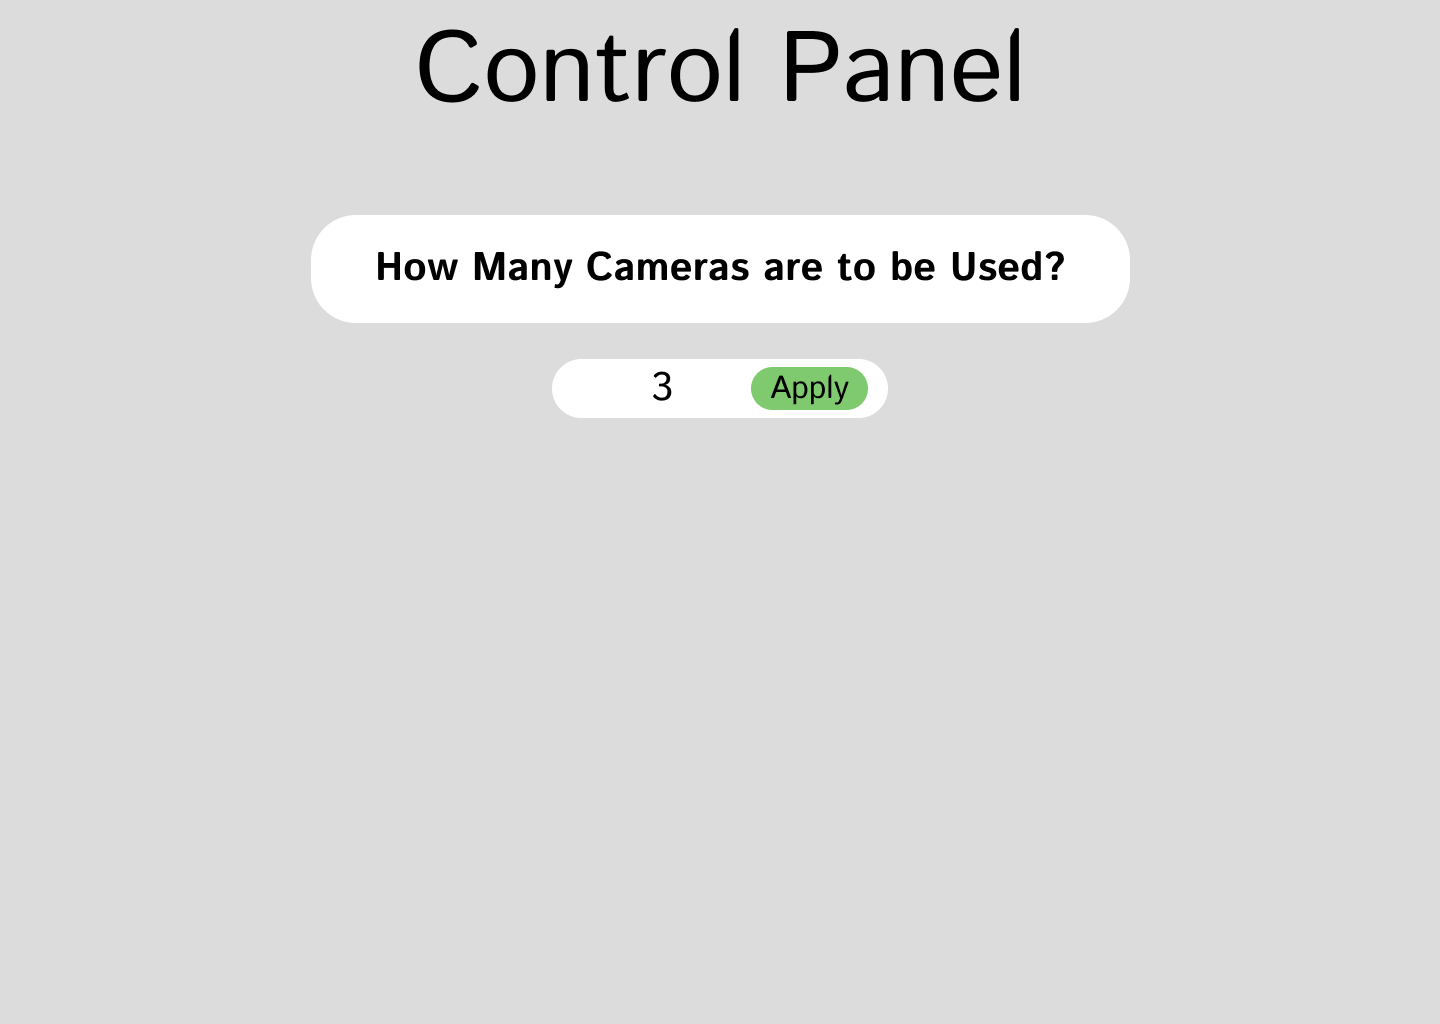
\includegraphics[width=\linewidth]{figures/methods/wireframes/control-panel-1.png}
        \caption{Step 1}
        \label{fig:control-panel-1}
    \end{subfigure}
    \hfill
    \begin{subfigure}[h!]{0.40\linewidth}
        \centering
        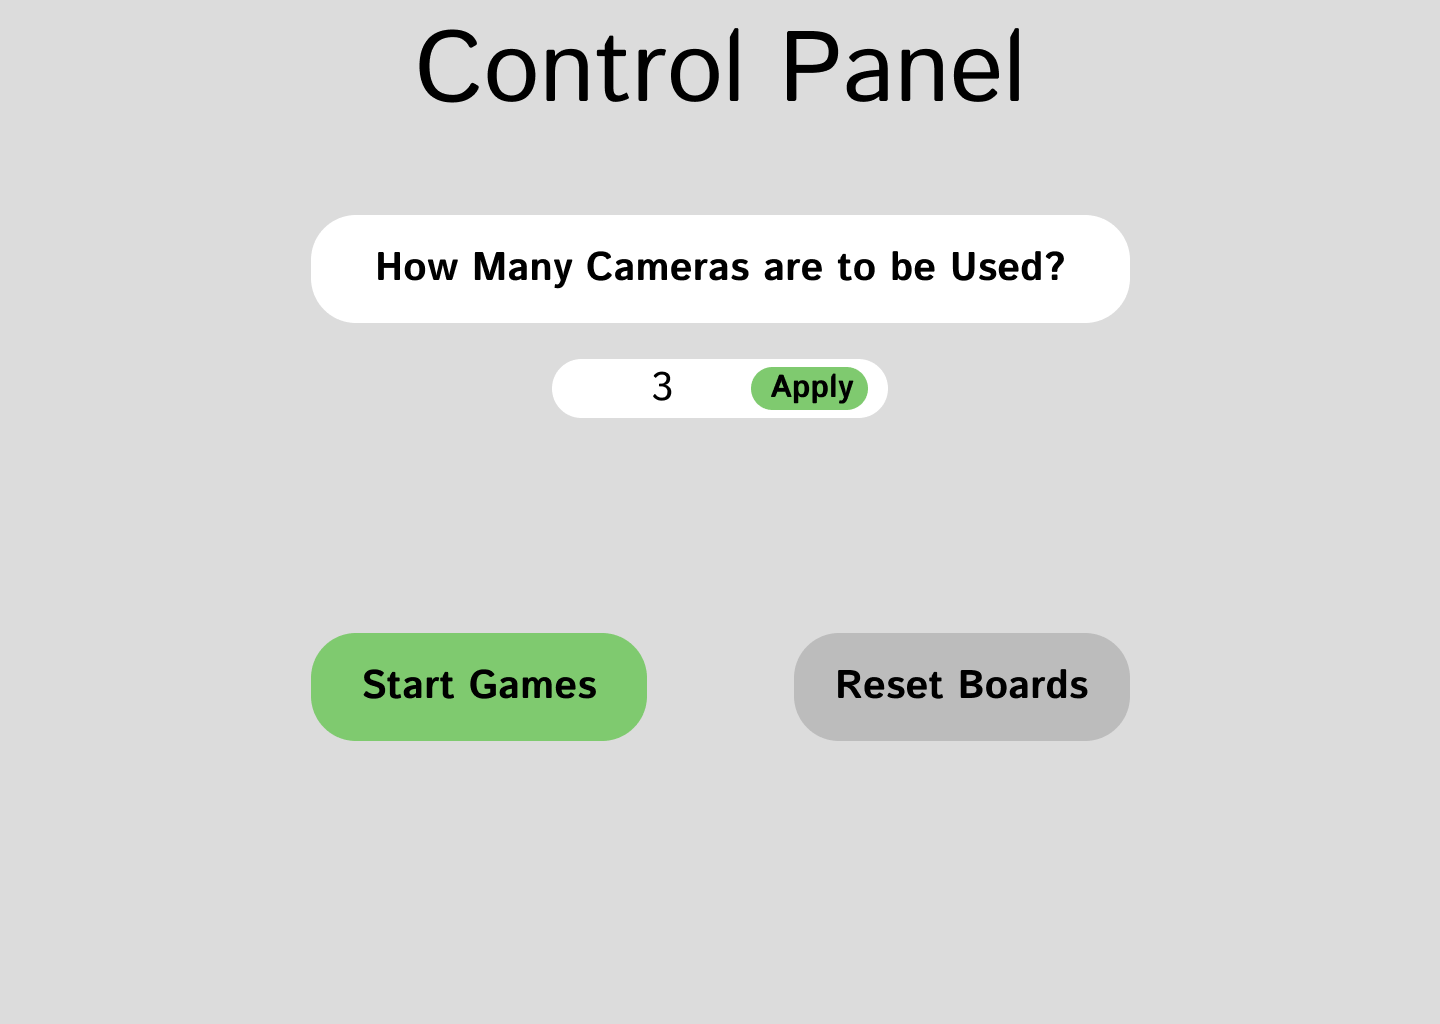
\includegraphics[width=\linewidth]{figures/methods/wireframes/control-panel-2.png}
        \caption{Step 2}
        \label{fig:control-panel-2}
    \end{subfigure}

    \begin{subfigure}[h!]{0.40\linewidth}
        \centering
        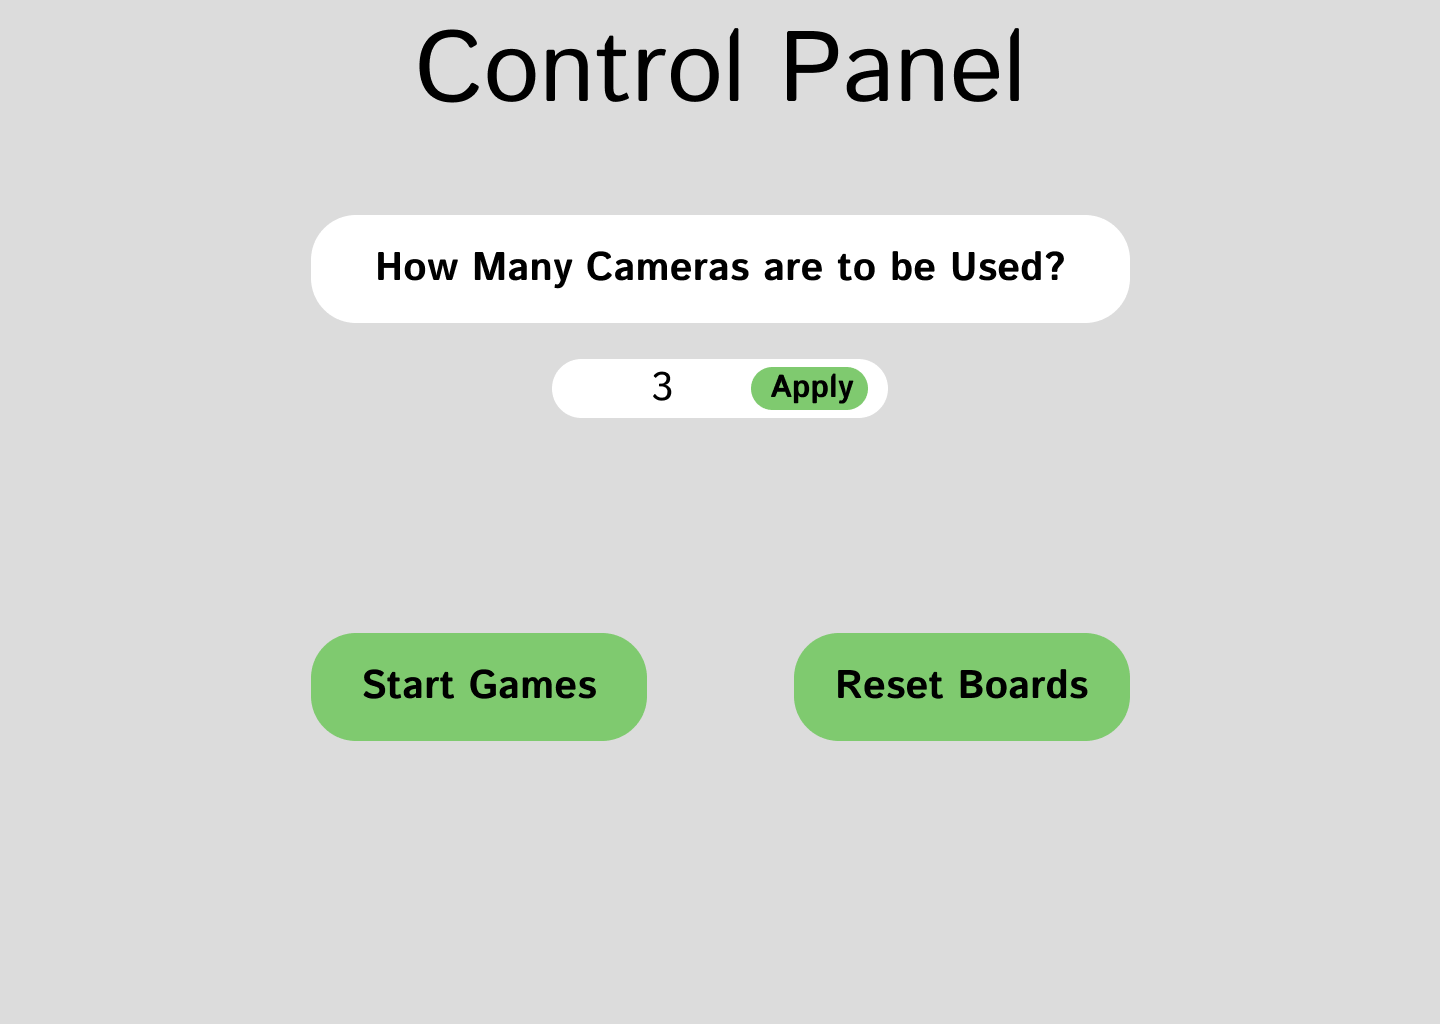
\includegraphics[width=\linewidth]{figures/methods/wireframes/control-panel-3.png}
        \caption{Step 3}
        \label{fig:control-panel-3}
    \end{subfigure}
    
    \caption[Control panel wireframes]{Control Panel wireframes showing sequential interaction steps.}
    \label{fig:control-panel-group}
\end{figure}


The client-side view is implemented as a web-based interface, developed in accordance with the accessibility principles described in Section \ref{sec:design}. The design prioritizes usability, aiming to offer a user-friendly and accessible experience for users across both desktop and mobile platforms. The interface is organized into two primary components: the Tournament View and the Board View. \\

The \textbf{Tournament View} (see Figure \ref{fig:desktop-tournament-view}) provides a concise overview of all active games in the tournament. Its clean and minimal layout presents key information such as board numbers, player names, and a navigation button for accessing the corresponding Board View. This approach ensures that users can quickly scan through the tournament and access gameswith minimal effort. \\

The \textbf{Board View} (see Figure \ref{fig:desktop-board-view}) is focused on a single game, displaying both the live chessboard and a video stream of the ongoing game. The layout is designed for clarity, minimizing distractions so that users can easily follow the game in progress. \\

To ensure compatibility with mobile devices, the interface incorporates responsive design principles. On smaller screens, the Tournament View simplifies its presentation by removing player names and retaining only the board number and navigation button (see Figure \ref{fig:phone-tournament-view}). This streamlined layout maintains usability without overwhelming the limited screen space.
Similarly, the Board View adjusts to a vertical layout on mobile devices, stacking the chessboard and video stream one above the other (see Figure \ref{fig:phone-board-view}). This configuration enhances readability and preserves the overall clarity of the interface, even on compact displays.


\begin{figure}[h!]
\subsubsection*{Desktop View}
    \centering
    \begin{subfigure}[h!]{0.40\linewidth}
        \centering
        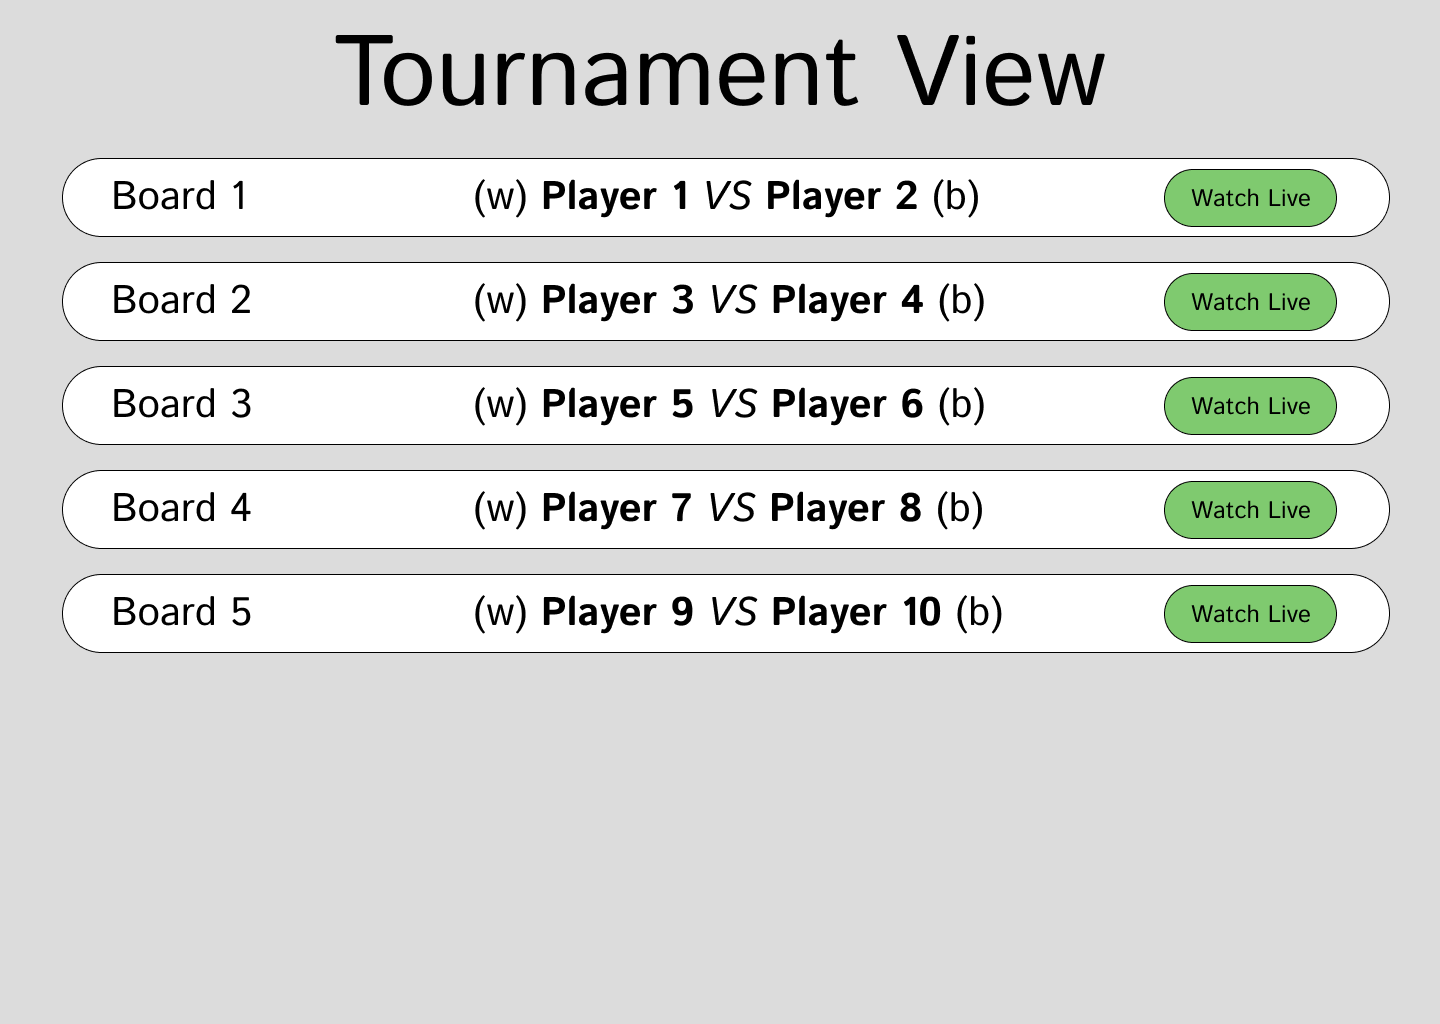
\includegraphics[width=\linewidth]{figures/methods/wireframes/desktop-tournament-view.png}
        \caption{Tournament View}
        \label{fig:desktop-tournament-view}
    \end{subfigure}
    \hfill
    \begin{subfigure}[h!]{0.40\linewidth}
        \centering
        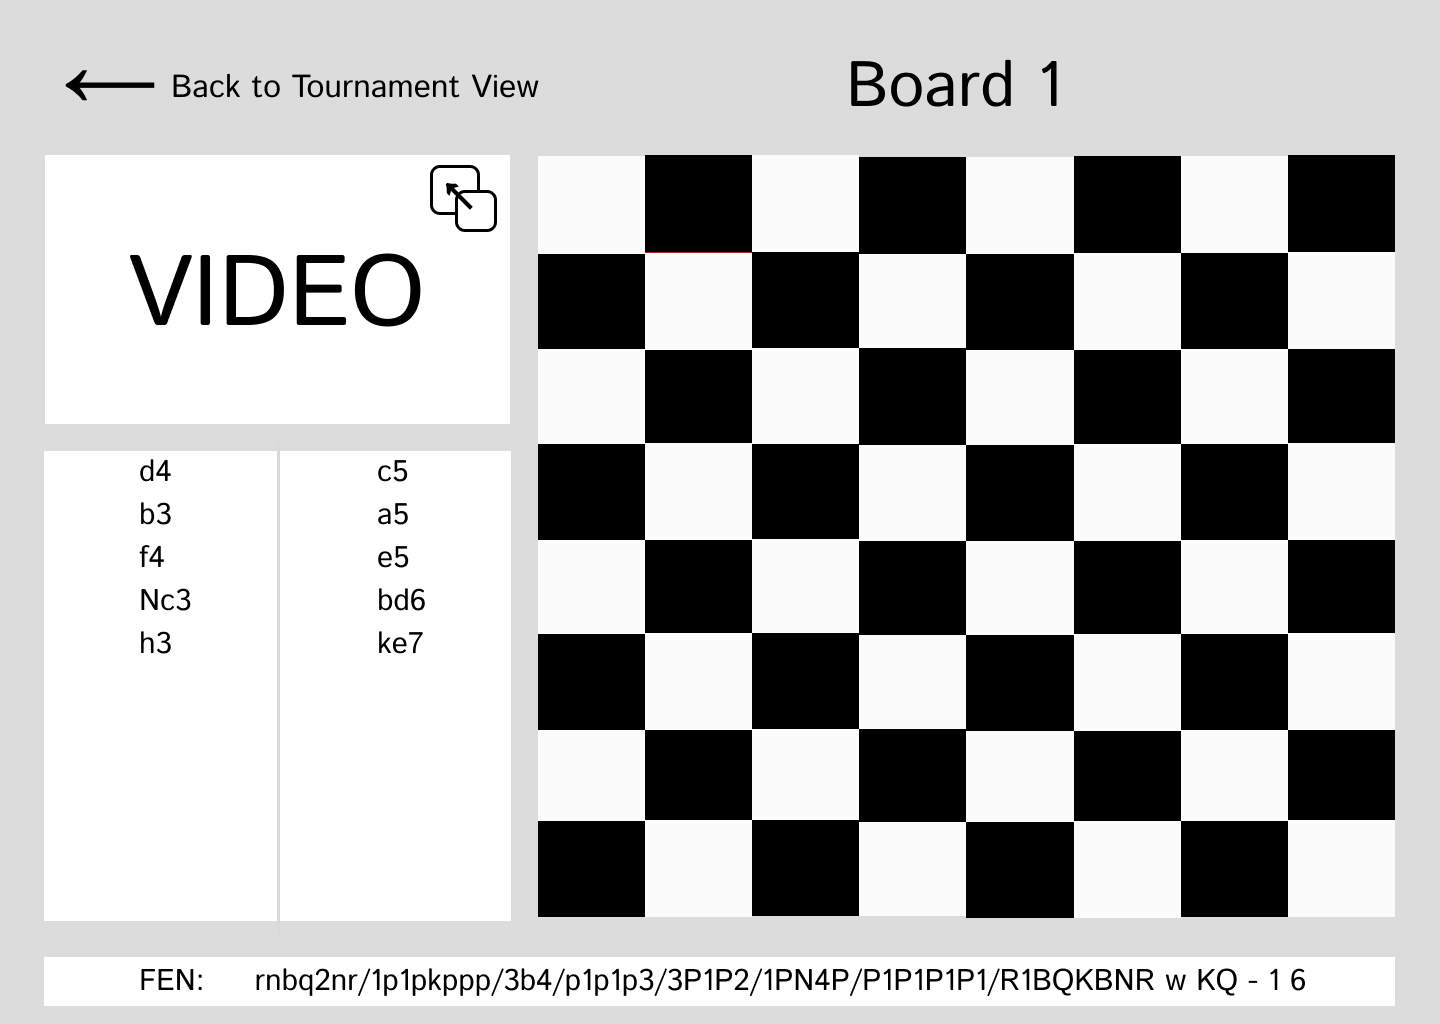
\includegraphics[width=\linewidth]{figures/methods/wireframes/desktop-board-view.png}
        \caption{Board View}
        \label{fig:desktop-board-view}
    \end{subfigure}

    \begin{subfigure}[h!]{0.40\linewidth}
        \centering
        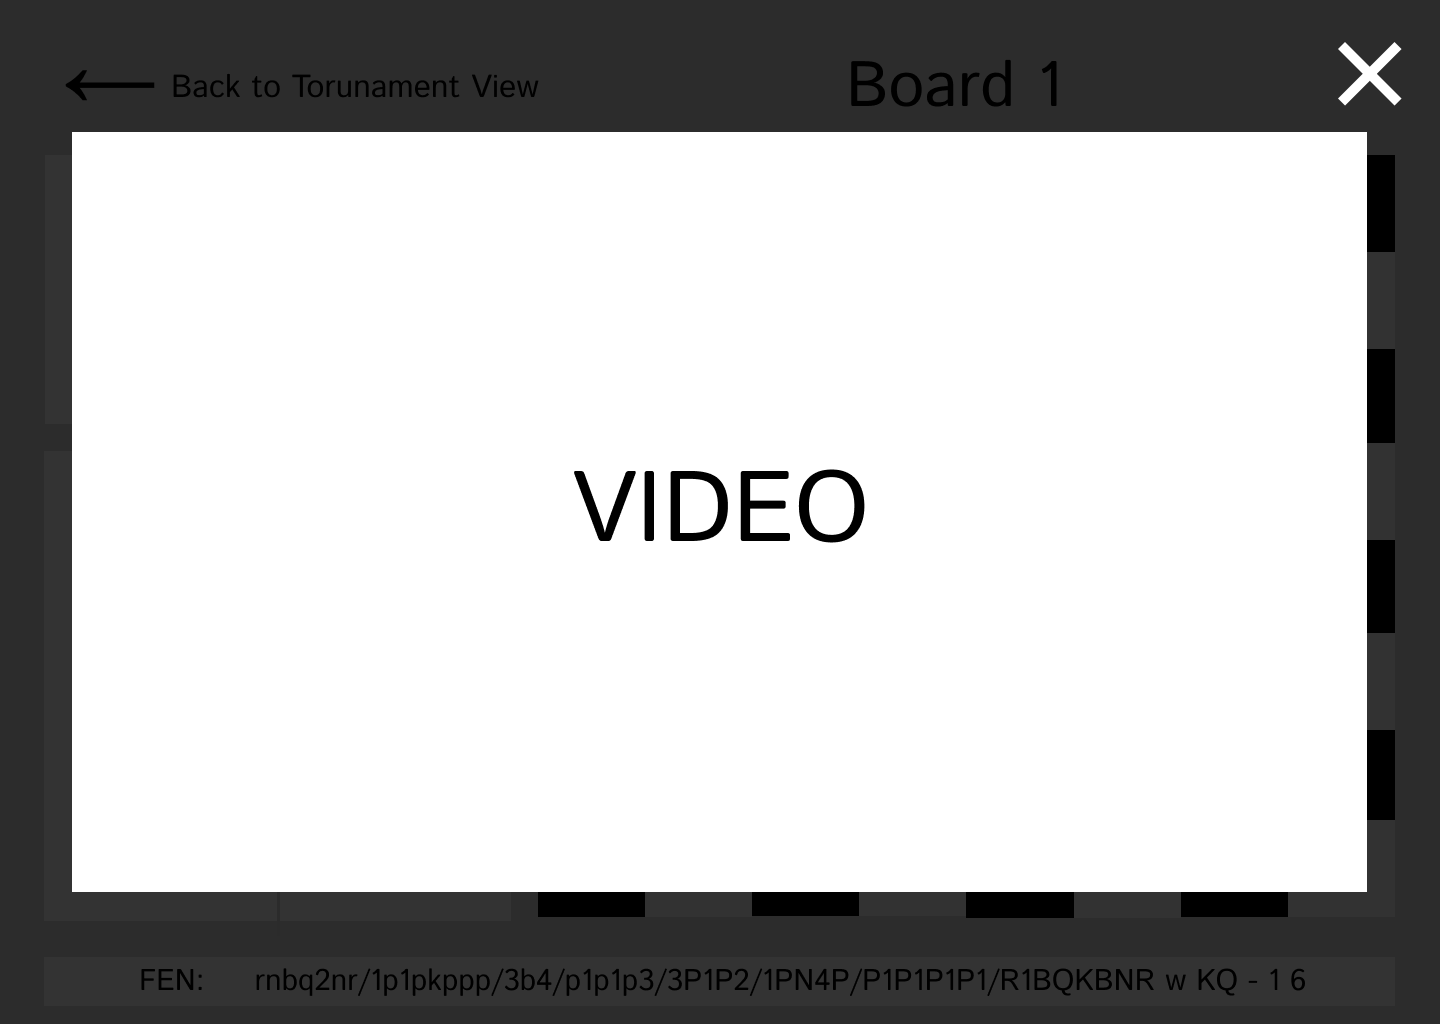
\includegraphics[width=\linewidth]{figures/methods/wireframes/desktop-full-screen-video-view.png}
        \caption{Fullscreen Video Feed}
        \label{fig:desktop-fullscreen-video}
    \end{subfigure}
    
    \caption{Desktop client-side wireframes}
    \label{fig:desktop-view-group}
\end{figure}


\begin{figure}[h!]
\subsubsection*{Phone View}
    \centering
    \begin{subfigure}[h!]{0.2\linewidth}
        \centering
        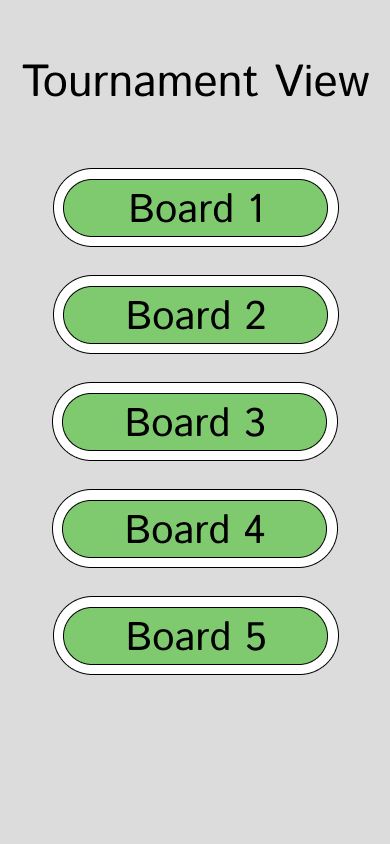
\includegraphics[width=\linewidth]{figures/methods/wireframes/phone-tournament-view.png}
        \caption{Tournament View}
        \label{fig:phone-tournament-view}
    \end{subfigure}
    \hfill
    \begin{subfigure}[h!]{0.2\linewidth}
        \centering
        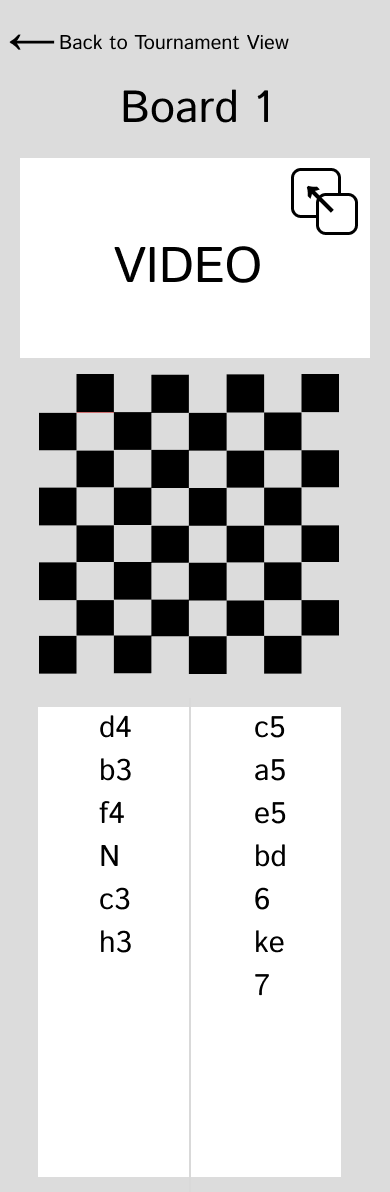
\includegraphics[width=\linewidth]{figures/methods/wireframes/phone-board-view.png}
        \caption{Board View}
        \label{fig:phone-board-view}
    \end{subfigure}
    \hfill
    \begin{subfigure}[h!]{0.2\linewidth}
        \centering
        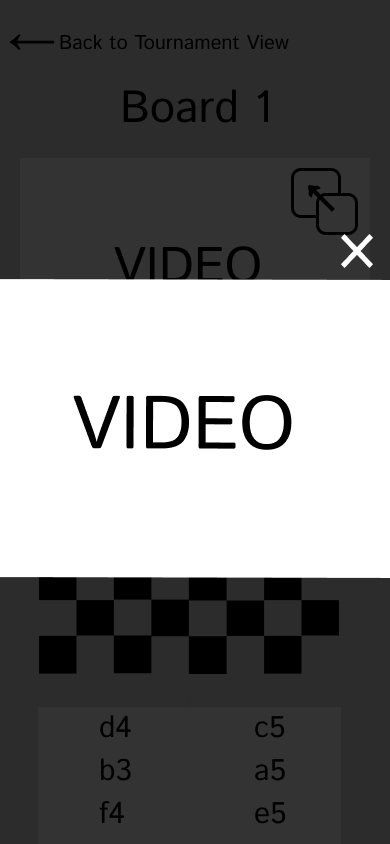
\includegraphics[width=\linewidth]{figures/methods/wireframes/phone-full-screen-video-view-vertical.png}
        \caption{Vertical Fullscreen Video Feed}
        \label{fig:phone-fullscreen-video-vertical}
    \end{subfigure}
    \hfill
    \begin{subfigure}[h!]{0.2\linewidth}
        \centering
        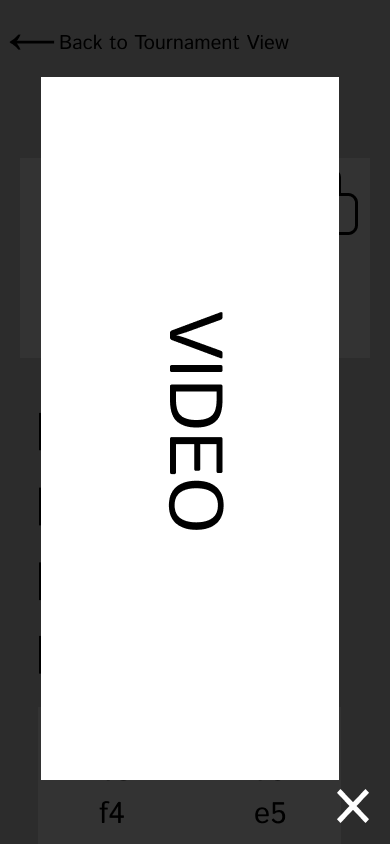
\includegraphics[width=\linewidth]{figures/methods/wireframes/phone-full-screen-video-view-horizontal.png}
        \caption{Horizontal Fullscreen Video Feed}
        \label{fig:phone-fullscreen-video-horizontal}
    \end{subfigure}
    
    \caption{Phone client-side wireframes}
    \label{fig:phone-view-group}
\end{figure}

\newpage

\section{Project management}
\label{sec:methods-project-management}
The team adopted the \gls{scrum} framework to organize the project and coordinate tasks effectively. Work was divided into biweekly sprints, each beginning with a planning session where prioritized items were selected from the product backlog. Tasks were then broken down into manageable units and assigned to individual team members. The sprint goals guided the development process, culminating in a sprint review and retrospective at the end of each cycle to assess outcomes and reflect on team performance. \\

To support this workflow, a meeting routine was established. Internal team meetings were held as needed to discuss progress, resolve blockers, and coordinate efforts. Additionally, brief informal stand-up meetings took place during office hours to maintain shared awareness of current tasks and priorities. Biweekly meetings with the supervisor ensured ongoing guidance and alignment with academic requirements. Meetings with the product owner occurred approximately once or twice per month, providing opportunities to present progress and gather valuable feedback. \\

To support effective collaboration, responsibilities were divided among team members. Roles included communication lead, meeting minute writer, and documentation manager. The distribution of roles helped maintain a consistent workflow and ensured accountability across different project areas. All meeting minutes were documented and stored in the project repository alongside the main report. Sprint reviews, retrospectives, and other supplementary documentation, including the project timetable, testing data, and contact log, were maintained in a shared OneDrive folder. \\

Communication was primarily facilitated through Discord, which served as the team's communication platform. This included informal discussions and quick coordination on tasks and meeting times within the team. Email was used for formal communication and documentation, such as scheduling meetings with the supervisor or product owner. \\

GitHub was used for both version control and task management. Issues in GitHub were used to define and track units of work. These were categorized and organized using labels. Each issue could be assigned, prioritized, and monitored through a visual interface. GitHub pull requests also enabled peer review of code contributions before integration. All code contributions and associated tasks were managed through GitHub's branching model. This allowed team members to work independently on features and bugs, while maintaining a clean and stable main branch. \\

\section{Tools and Platforms}
\label{sec:tools-and-platforms}

\subsection*{Development Tools}
\label{subsec:development-tools}

\begin{itemize}
    \item \textbf{\acrlong{vscode}} was used as the primary development environment due to its support for multiple programming languages and extensions.
\item \textbf{Postman} was employed for testing and validating \acrshort{rest}ful \glspl{api}, utilizing built-in JavaScript-based test snippets.
\item \textbf{Netron.app} was used to visualize neural network architectures during the evaluation phase.
\item \textbf{Git} facilitated version control and collaboration throughout the development process.
\item \textbf{\glspl{llm}} (for example ChatGPT) were consulted to review code and provide suggestions, functioning as a collaborative assistant.
\item \textbf{Lighthouse} was used to evaluate and improve the performance and accessibility of the developed web interface.
\end{itemize}.

\subsection*{Collaboration Tools}
\label{subsec:collaboration-and-design-tools}

\begin{itemize}
    \item \textbf{GitHub} was used for its integrated project management features, enabling the team to create an Issue Board for efficient tracking of tasks. It was also used for code reviews and version control.

    \item \textbf{Figma} was used as a tool for sketching and creating wireframes.
    
    \item \textbf{OneDrive} was used as a platform for storing and sharing files.
    
    \item \textbf{Overleaf} was used as the platform for writing the report, utilizing its LaTeX support to efficiently compose and format the thesis.
\end{itemize}

\newpage

\section{Technology Stack}
\label{sec:technology-stack}

\subsection*{Backend}

Python was selected for the project’s backend because of its simple and user-friendly syntax. Its extensive ecosystem of libraries and frameworks reduces development time. Furthermore, Python’s community and industry provide valuable resources for \gls{api} development and \gls{ml} capabilities.

\subsubsection*{Python Libraries}

\begin{itemize}
    \item \textbf{chess} - Used for move generation, validation, and parsing of chess game formats \cite{python:chess}.
    \item \textbf{FastAPI} - Web framework used to develop \acrshort{rest}ful \glspl{api} for backend services \cite{python:fastapi}.
    \item \textbf{numpy} - Package for numerical operations \cite{python:numpy}.
    \item \textbf{onnxruntime} - Used for running pre-trained machine learning models \cite{python:onnx}.
    \item \textbf{opencv-python} - Utilized for computer vision tasks \cite{python:opencv}.
    \item \textbf{requests} - Used to handle \gls{http} communication \cite{python:requests}.
    \item \textbf{scipy} – Employed for scientific and numerical computations \cite{python:scipy}.
    \item \textbf{tensorflow} - Used to build and execute \gls{ml} models \cite{python:tensorflow}.
    \item \textbf{customtkinter} - Desktop \gls{ui} built with a modern Tkinter-based library offering customizable widgets. \cite{python:ctk}
\end{itemize}


\subsection*{Frontend}

TypeScript was selected for the project's frontend language due to it's type-safety, as discussed in Section \ref{subsec:type-safety}.

\subsubsection*{TypeScript Dependencies}

\begin{itemize}
    \item \textbf{Vite} - A fast frontend build tool for web applications \cite{ts:vite}.
    
    \item \textbf{React} - Builds user interfaces from individual pieces called components \cite{ts:react}.
    
    \item \textbf{\acrshort{swc}} - Speeds up the Vite development server \cite{ts:swc}.
    
    \item \textbf{chess.ts} - A TypeScript chess library for handling game logic including move validation and piece management \cite{ts:chess}.
    
    \item \textbf{react-dom} - Serves as the entry point to the DOM and server renderers for React \cite{ts:react-dom}.
\end{itemize}

\newpage

\section{Testing}
\label{sec:testing}

\subsection{Model testing}
\label{subsec:model-testing}
The performance of the machine learning model was evaluated through 100 test  games. Five distinct chess openings were selected, with 10 games played per opening on each of two board types: plastic and wooden. This resulted in 50 games per board type. Each game consisted of 15 full moves, corresponding to 15 moves by white and 15 moves by black. \\

Each move was logged as either successful or unsuccessful. A 30-second window was provided for the model to detect and transmit each move, starting from the moment the move was made \gls{otb}. If the model failed to detect the move within this time frame, or if it detected the wrong move, it was marked as unsuccessful. The game concluded either when a move was marked unsuccessful or all 15 full moves had been completed. \\

The webcam was mounted above the board at an angle of approximately 60–70\si{\degree} relative to the table surface. The white pieces were placed on the left side of the camera's field of view, and the black pieces on the right.

\begin{figure}[h!]
    \centering
    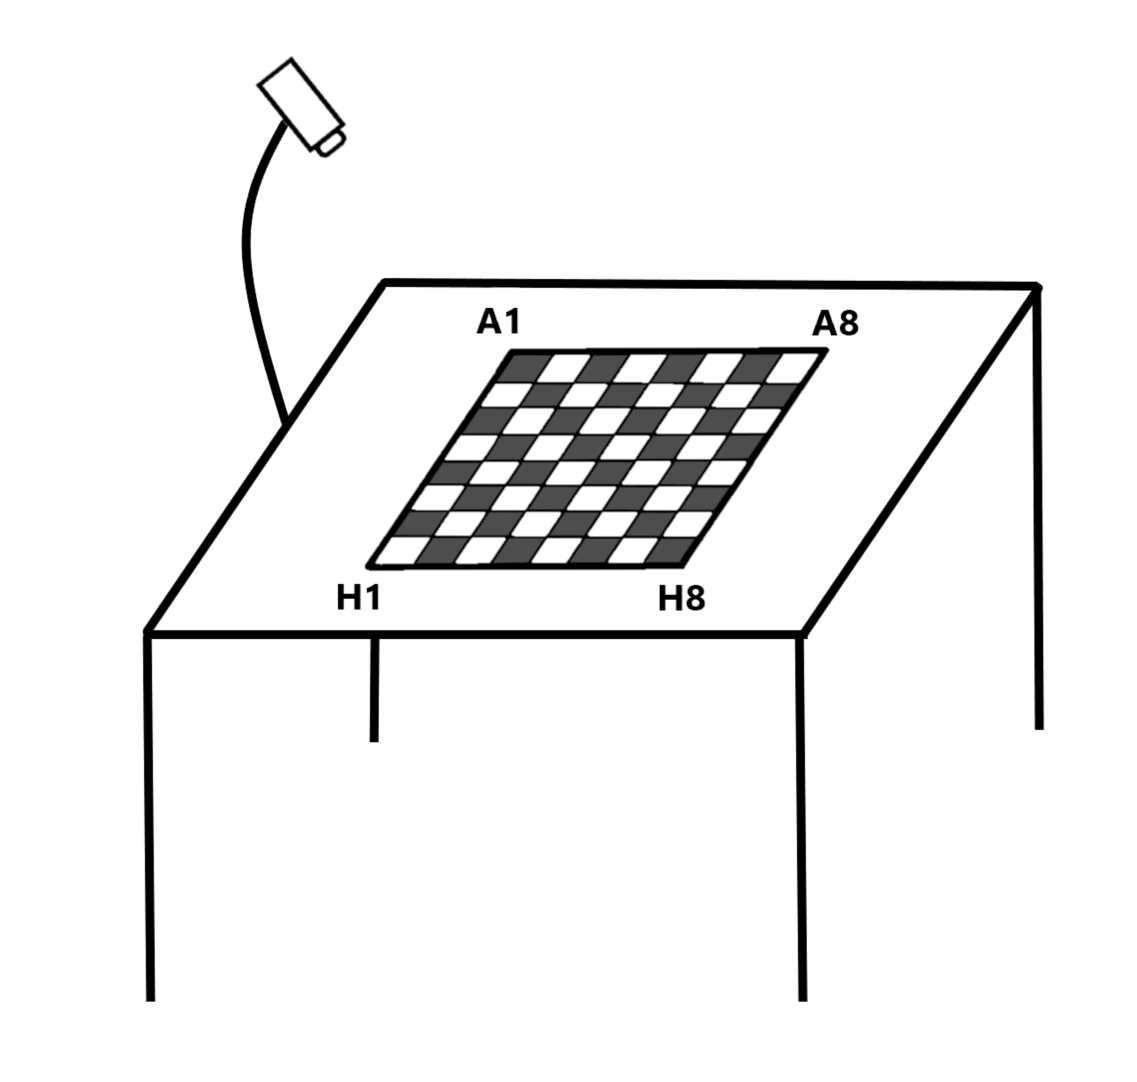
\includegraphics[width=0.65\linewidth]{figures/methods/testing/setup.png}
    \caption[Setup during testing]{Physical setup during testing, showing the board, camera position, and piece orientation.}
    \label{fig:setup}
\end{figure}

\newpage

\subsection{API}
\label{subsec:api-methods}

\subsubsection*{WebSocket Testing (Live Data Simulation)}
\label{subsubsec:websocket-methods}

To test real-time communication via WebSocket, a lightweight simulator was implemented. The simulator sequentially sent hard-coded chess moves to connected clients, emulating live gameplay data. The frontend application was connected to the WebSocket endpoint during testing, enabling it to receive and display incoming data. This setup allowed for effective verification of the WebSocket functionality and ensured that the frontend was capable of handling and rendering live move updates as intended.

\subsubsection*{REST API Testing with Postman}
\label{subsubsec:rest-api-methods}

To verify the correctness of the \gls{rest}ful \gls{api} endpoints, Postman was used as a manual testing tool. Postman enables direct interaction with \gls{http} endpoints, making it well-suited for verifying both request structures and server responses. Each implemented endpoint was tested individually, including operations such as resetting specific boards, resetting all boards simultaneously, retrieving the list of active boards, and streaming video from individual board cameras. \\

Figure~\ref{fig:postman-rest-tests} illustrates sample \gls{api} calls tested through Postman. Various \texttt{POST} and \texttt{GET} requests were issued to endpoints such as \texttt{/reset/1}, \texttt{/video/1}, and \texttt{/boards}. These tests confirmed that backend services responded as expected, returning successful status codes, valid response payloads, and triggering the intended state changes. This form of manual \gls{rest} testing ensured \gls{api} correctness prior to frontend integration.

\begin{figure}[h!]
    \centering
    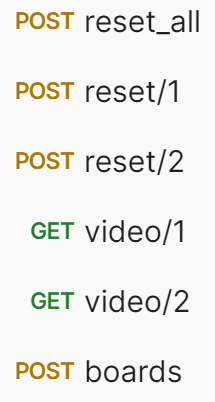
\includegraphics[width=0.25\linewidth]{figures//methods/postman-light.png}
    \caption[Postman REST API Tests]{Postman \gls{rest} \gls{api} Tests}
    \label{fig:postman-rest-tests}
\end{figure}

\subsection{Wireframe testing}
\label{subsubsec:user-centered-design}

The usability testing process followed principles discussed in Section \ref{subsec:testing}. At the early stage of the design process, wireframe testing was conducted with a small but diverse group of users. The aim was to evaluate whether the interface was intuitive, and whether the sizing and layout were appropriate for a range of users. \\

Participants included individuals from various age groups (ranging from 18 to 55) and backgrounds, including both experienced chess players and those unfamiliar with the game. Their technical experience also varied, from computer science students to non-technical individuals such as stay-at-home parents. In total, eight participants were involved in this test, excluding the developers and stakeholders of the project. \\

Before testing began, all participants were presented with the following scenario to establish context:

\begin{quote}
\textit{You are viewing a chess game between two companions you know. You visit the tournament organizer's website and come across this webpage.}
\end{quote}

Participants were then asked to either complete a set of predefined tasks or freely explore the interface, simulating a real-world browsing scenario. This approach was designed to assess how naturally users could navigate the interface without guidance. \\

After their interaction with the wireframe, participants completed an anonymous feedback form, which included the following questions:

\begin{itemize}
    \item \textit{On a scale from 1 to 5, how satisfied are you with the overall experience of the application?}
    \item \textit{On a scale from 1 to 5, how satisfied are you with the Tournament View page?}
    \item \textit{On a scale from 1 to 5, how satisfied are you with the Board View page?}
    \item \textit{Do you have any feedback, suggestions for improvement, or features you would like to see added?}
\end{itemize}

See Section \ref{subsec:wireframe} for the final tested wireframe.



\subsection{Color palette testing}
\label{subsubsec:color-palette}

In selecting the application’s color palette, the group opted for a variation of blue. This choice was influenced by the symbolic associations of the color blue, which is linked to imagination, intelligence, and wisdom \cite{blue}. These are traits that are relevant to the game of chess \cite{chess:ppqty, chess:chess-and-creativity}. \\

To identify the most suitable stylistic direction, several versions of the application were developed, each featuring a distinct color palette. These prototypes were printed and displayed in a shared space, allowing individuals from diverse backgrounds to view and compare them. Participants were invited to vote for their preferred versions through a form. Each participant was allowed up to three votes and had the option to leave comments.